\documentclass[a4paper,10pt]{article}

\usepackage[T1]{fontenc}
\usepackage[utf8]{inputenc}
\usepackage{graphicx}
\usepackage{xcolor}
\usepackage{fourier}
\usepackage{caption}
\usepackage{subcaption}
\usepackage{cprotect}

\usepackage{tgtermes}

\usepackage[
pdftitle={Statistical Machine Learning}, 
pdfauthor={Inez Wijnands \& Guido Zuidhof, Radboud University Nijmegen},
colorlinks=true,linkcolor=blue,urlcolor=blue,citecolor=blue,bookmarks=true,
bookmarksopenlevel=2]{hyperref}
\usepackage{amsmath,amssymb,amsthm,textcomp}
\usepackage{enumerate}
\usepackage{multicol}
\usepackage{tikz}

\usepackage{geometry}
\geometry{total={210mm,297mm},
left=25mm,right=25mm,%
bindingoffset=0mm, top=20mm,bottom=20mm}

\numberwithin{equation}{section} % Number equations within sections (i.e. 1.1 instead of 1)
\numberwithin{figure}{section} % Number figures within sections (i.e. 1.1 i/o 1)
\numberwithin{table}{section} % Number tables within sections (i.e. 1.1 i/of 1)

\linespread{1.35}

\newcommand{\linia}{\rule{\linewidth}{0.5pt}}

% custom theorems if needed
\newtheoremstyle{mytheor}
    {1ex}{1ex}{\normalfont}{0pt}{\scshape}{.}{1ex}
    {{\thmname{#1 }}{\thmnumber{#2}}{\thmnote{ (#3)}}}

\theoremstyle{mytheor}
\newtheorem{defi}{Definition}

% my own titles
\makeatletter
\renewcommand{\maketitle}{
\begin{center}
\vspace{2ex}
{\huge \textsc{\@title}}
\vspace{1ex}
\\
\linia\\
\@author  \@date
\vspace{4ex}
\end{center}
}
\makeatother
%%%

% custom footers and headers
\usepackage{fancyhdr,lastpage}
\pagestyle{fancy}
\lhead{}
\chead{}
\rhead{}
\lfoot{Assignment \textnumero{} 3}
\cfoot{}
\rfoot{Page \thepage\ /\ \pageref*{LastPage}}
\renewcommand{\headrulewidth}{0pt}
\renewcommand{\footrulewidth}{0pt}
%

% code listing settings
\usepackage{listings}
\lstset{
    language=Python,
    basicstyle=\ttfamily\small,
    aboveskip={0.9\baselineskip},
    belowskip={0.9\baselineskip},
    columns=fixed,
    extendedchars=true,
    breaklines=true,
    tabsize=4,
    prebreak=\raisebox{0ex}[0ex][0ex]{\ensuremath{\hookleftarrow}},
    frame=lines,
    showtabs=false,
    showspaces=false,
    showstringspaces=false,
    keywordstyle=\color[rgb]{0.1,0.126,0.941},
    commentstyle=\color[rgb]{0.133,0.545,0.133},
    stringstyle=\color[rgb]{0,0.5,0},
    numbers=left,
    numberstyle=\scriptsize\ttfamily,
    stepnumber=1,
    numbersep=10pt,
    captionpos=t,
    escapeinside={\%*}{*)}
}

%%%----------%%%----------%%%----------%%%----------%%%

\begin{document}

\title{Statistical Machine Learning \\ Assignment 3}

\author{Inez Wijnands (s4149696) \& Guido Zuidhof (s4160703)\\ Radboud University Nijmegen\\}

\date{03/12/2015}

\maketitle

\noindent \textit{The entire code listing is included in the zip-file. The listings shown here are merely code snippets}.\vspace{-0.5cm}
\section{Bayesian linear regression}
\begin{enumerate}
	\item 
	\item \begin{figure}[h!]
   			\centering
   			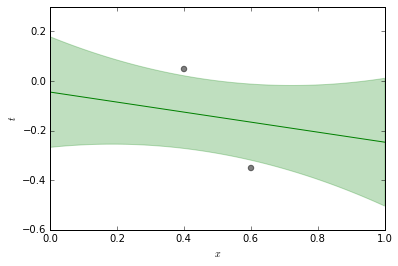
\includegraphics{exercise1plottanopink.png}\vspace{-0.4cm}
   			\caption{\vspace{-0.1cm} The mean of the predictive Gaussian distribution is represented by the green line, plotted against $x$. \vspace{-0.1cm}The two grey dots are the data points $\{x_1,t_1\}$ and $\{x_2,t_2\}$. The light green area indicates the standard deviation and is bound by the mean plus the standard deviationd and the mean minus the standard deviation.}\vspace{-0.2cm}
  		\end{figure}
	\item \begin{figure}[h!]
   			\centering
   			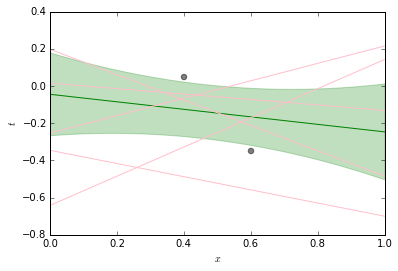
\includegraphics{exercise1plotta.png}\vspace{-0.4cm}
   			\caption{\vspace{-0.0cm} The pink lines represent $y(x,\boldsymbol{w})$ where the weights $\boldsymbol{w}$ are sampled from the posterior distribution with mean $m_N$ and variance $S_N$.}
  		\end{figure}
\end{enumerate}

\section{Logistic regression}
\subsection{The IRLS algorithm}
\begin{enumerate}
	\item 
	\item 
	\item 
\end{enumerate}

\subsection{Two-class classification using logistic regression}
\begin{enumerate}
	\item 
\end{enumerate}
\end{document}
